\subsection{Tuning of ESKF for real data} \label{a2task3}
The next step was to see how the error state Kalman filter would perform on actual real life data. The available dataset contains IMU and GNSS measurements of a unmanned aerial vehicle (UAV) remotely controlled by an operator. The flight path of the UAV as seen from the GNSS measurements is shown in figure \ref{fig:real-track}.
\begin{figure}[H]
\centering
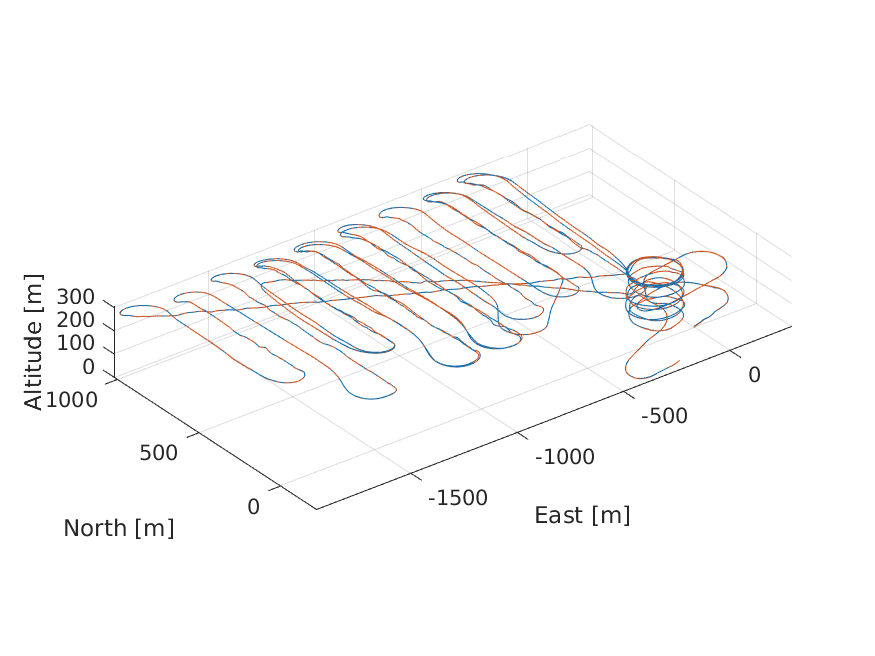
\includegraphics[width=0.6\textwidth]{plots/a2-real-track}
\caption{UAV Track for the real dataset. Red=GNSS measurements, Blue=ESKF}
\label{fig:real-track}
\end{figure}
With this real dataset, there are some other complications that must be adressed. First is the correction matrices $S_a$ and $S_g$ for the gyro and the accelerometer. These matrices correct for the orientation of the IMU in the body frame of the AUV. They also correct for misaligned axes IMU axes (that is, the IMU may be slightly malproduced with axes that are skewed somewhat off the orthogonal coordinate axes). These matrices however are of course not known exactly, because they are supposed to correct for unknown manufacturing errors, for this reason must expect some inaccuracy in the measurements. The second complication is the leverarm. This is the distance between the cener of control on the AUV and the mounting position of the IMU. This value has been measured and is given in the dataset. We give it as an input to the ESKF.

The tuning of the kalman filter model is again based on the STIM300 datasheet, as this is the actual IMU used on the UAV. The models acceleration noise $qA$ and gyro noise $qG$ were set by looking up the specification for velocity random walk and angular random walk respectively in the IMU datasheet and scaling it using $h = 3600s$ to get the correct unit ($[\frac{m}{s^2}$] and $[\frac{\circ}{s}]$). The gyro noise was also converted to radians. We tuned the bias models by hand, heavily inspired by our tuning from the simulated dataset. In this case, we do not have the ground truth available, so we cannot calculate the normalised error state squared (NEES). We are also not able to tune the filter using the error state. We can however use the \textit{innovation} of the kalman filter, which in layman terms is a measure of how much the filter must update or "innovate" the estimate in the update step to correct for the new measurement. In other words we can measure how "off" the prediction is which we further can compare with how certain the filter is when predicting. We also have the GNSS receivers estimated accuracy which we scaled and used as the standard deviation for the GNSS measurements. With our tuning, we are able to achieve a normalized innovation squared (NIS) that stays $82\%$ inside the $95\%$ $\chi^2$ confidence interval, shown in figure \ref{fig:nis_basic} below. We attempted to further tune the IMU noises, but decided it was better to use the official values provided by the manufacturer. Without ground truth and error metrics, it is difficult to further quantify the performance of the filter and it is difficult to further improve the tuning. 

\begin{figure}[H]
        \centering
        \begin{subfigure}[b]{0.45\textwidth}
                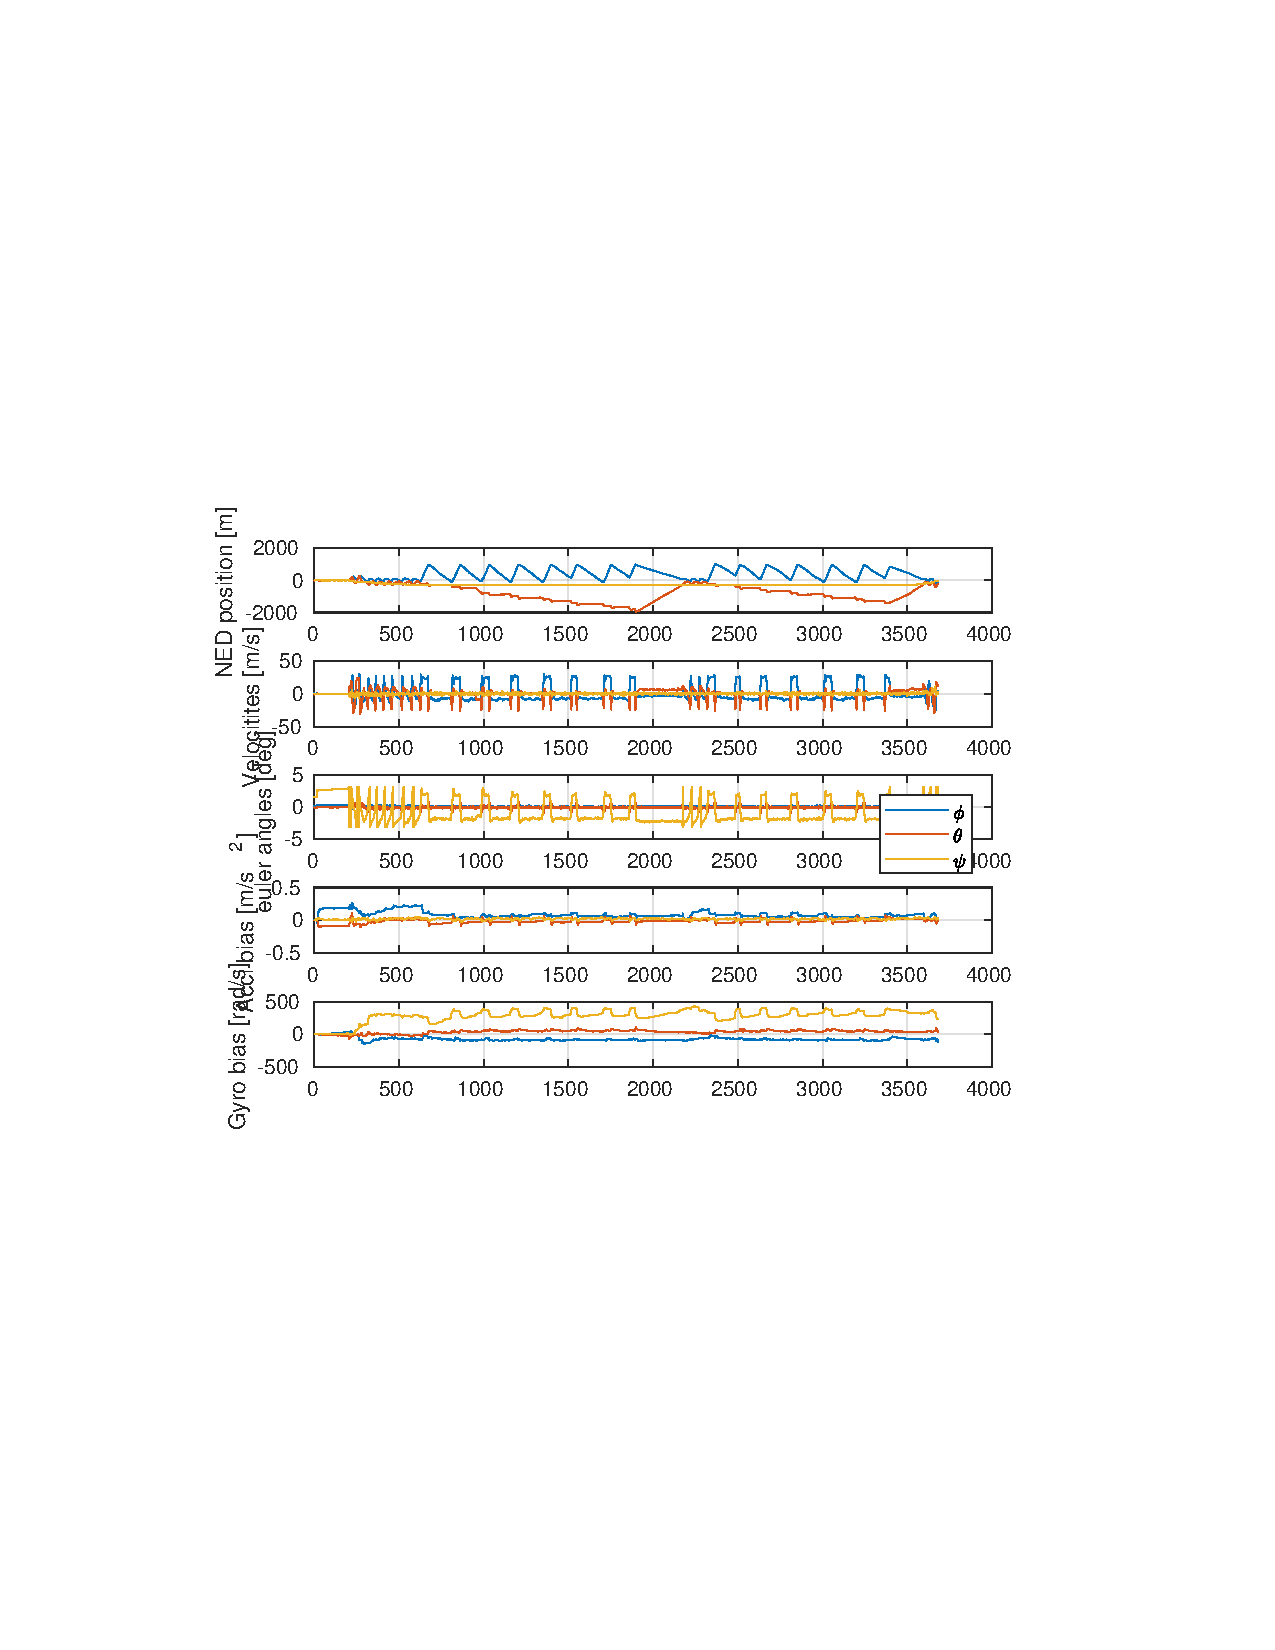
\includegraphics[width=\textwidth]{plots/a2-real-nis}
                \caption{NIS }
                \label{fig:nis_basic}
        \end{subfigure}%
~
        \begin{subfigure}[b]{0.45\textwidth}
                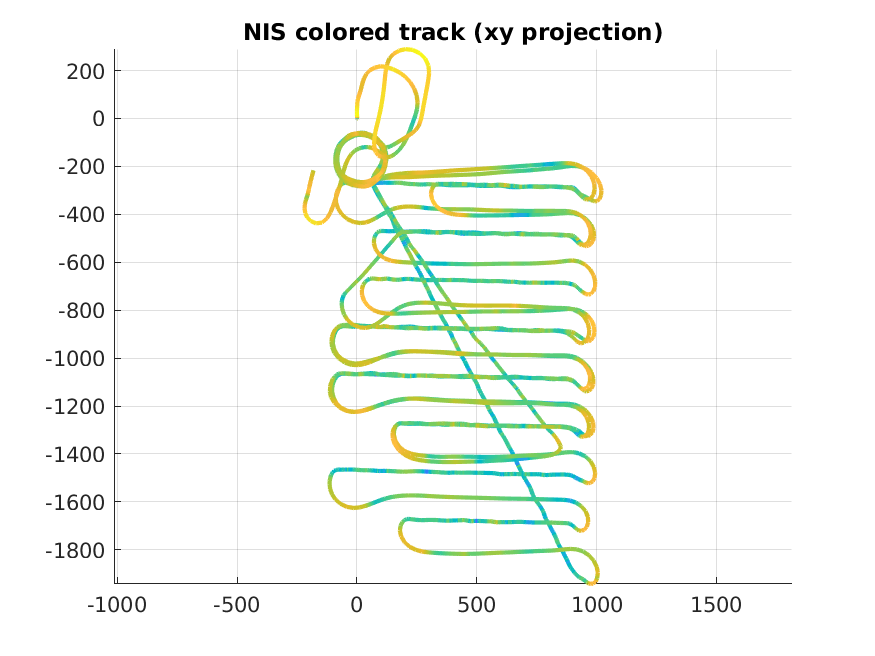
\includegraphics[width=\textwidth]{plots/a2-real-nis-colored-track}
                \caption{NIS colored track}
                \label{fig:nis_colored_track}
        \end{subfigure}
        \caption{Normalized Innovation Squared for the real dataset}
        \label{fig:nis}
\end{figure}

